\begin{frame}{Summary and Contributions}
  \begin{itemize}
    \pause
  \item Swarm/IoT has huge potentials but also challenges
    \pause
  \item Network resource adaptation
    \begin{itemize}
    \item Addresses scarce and variable WAN bandwidth
    \item Tradeoff between application accuracy and data size demand
    \end{itemize}

    \pause
  \item Compute resource adaptation
    \begin{itemize}
    \item Addresses heterogeneous platforms and large parameter space
    \item Tradeoff between application accuracy and processing times
    \end{itemize}

    \pause
  \item Overall, a systematic and quantitative approach for adaptation
  \end{itemize}
\end{frame}

\begin{frame}{Current (other) and Future Work}
  \footnotesize

  \vspace{1em}
  \metroset{block=fill}
  \begin{block}{TerraSwarm Vision}
    TerraSwarm applications are characterized by their ability to
    \alert{dynamically recruit} resources such as sensors and data from the
    cloud, aggregate and use that information to make or aid decisions.
  \end{block}

  \pause
  
  \begin{figure}
    \begin{subfigure}{0.49\textwidth}
      \centering
      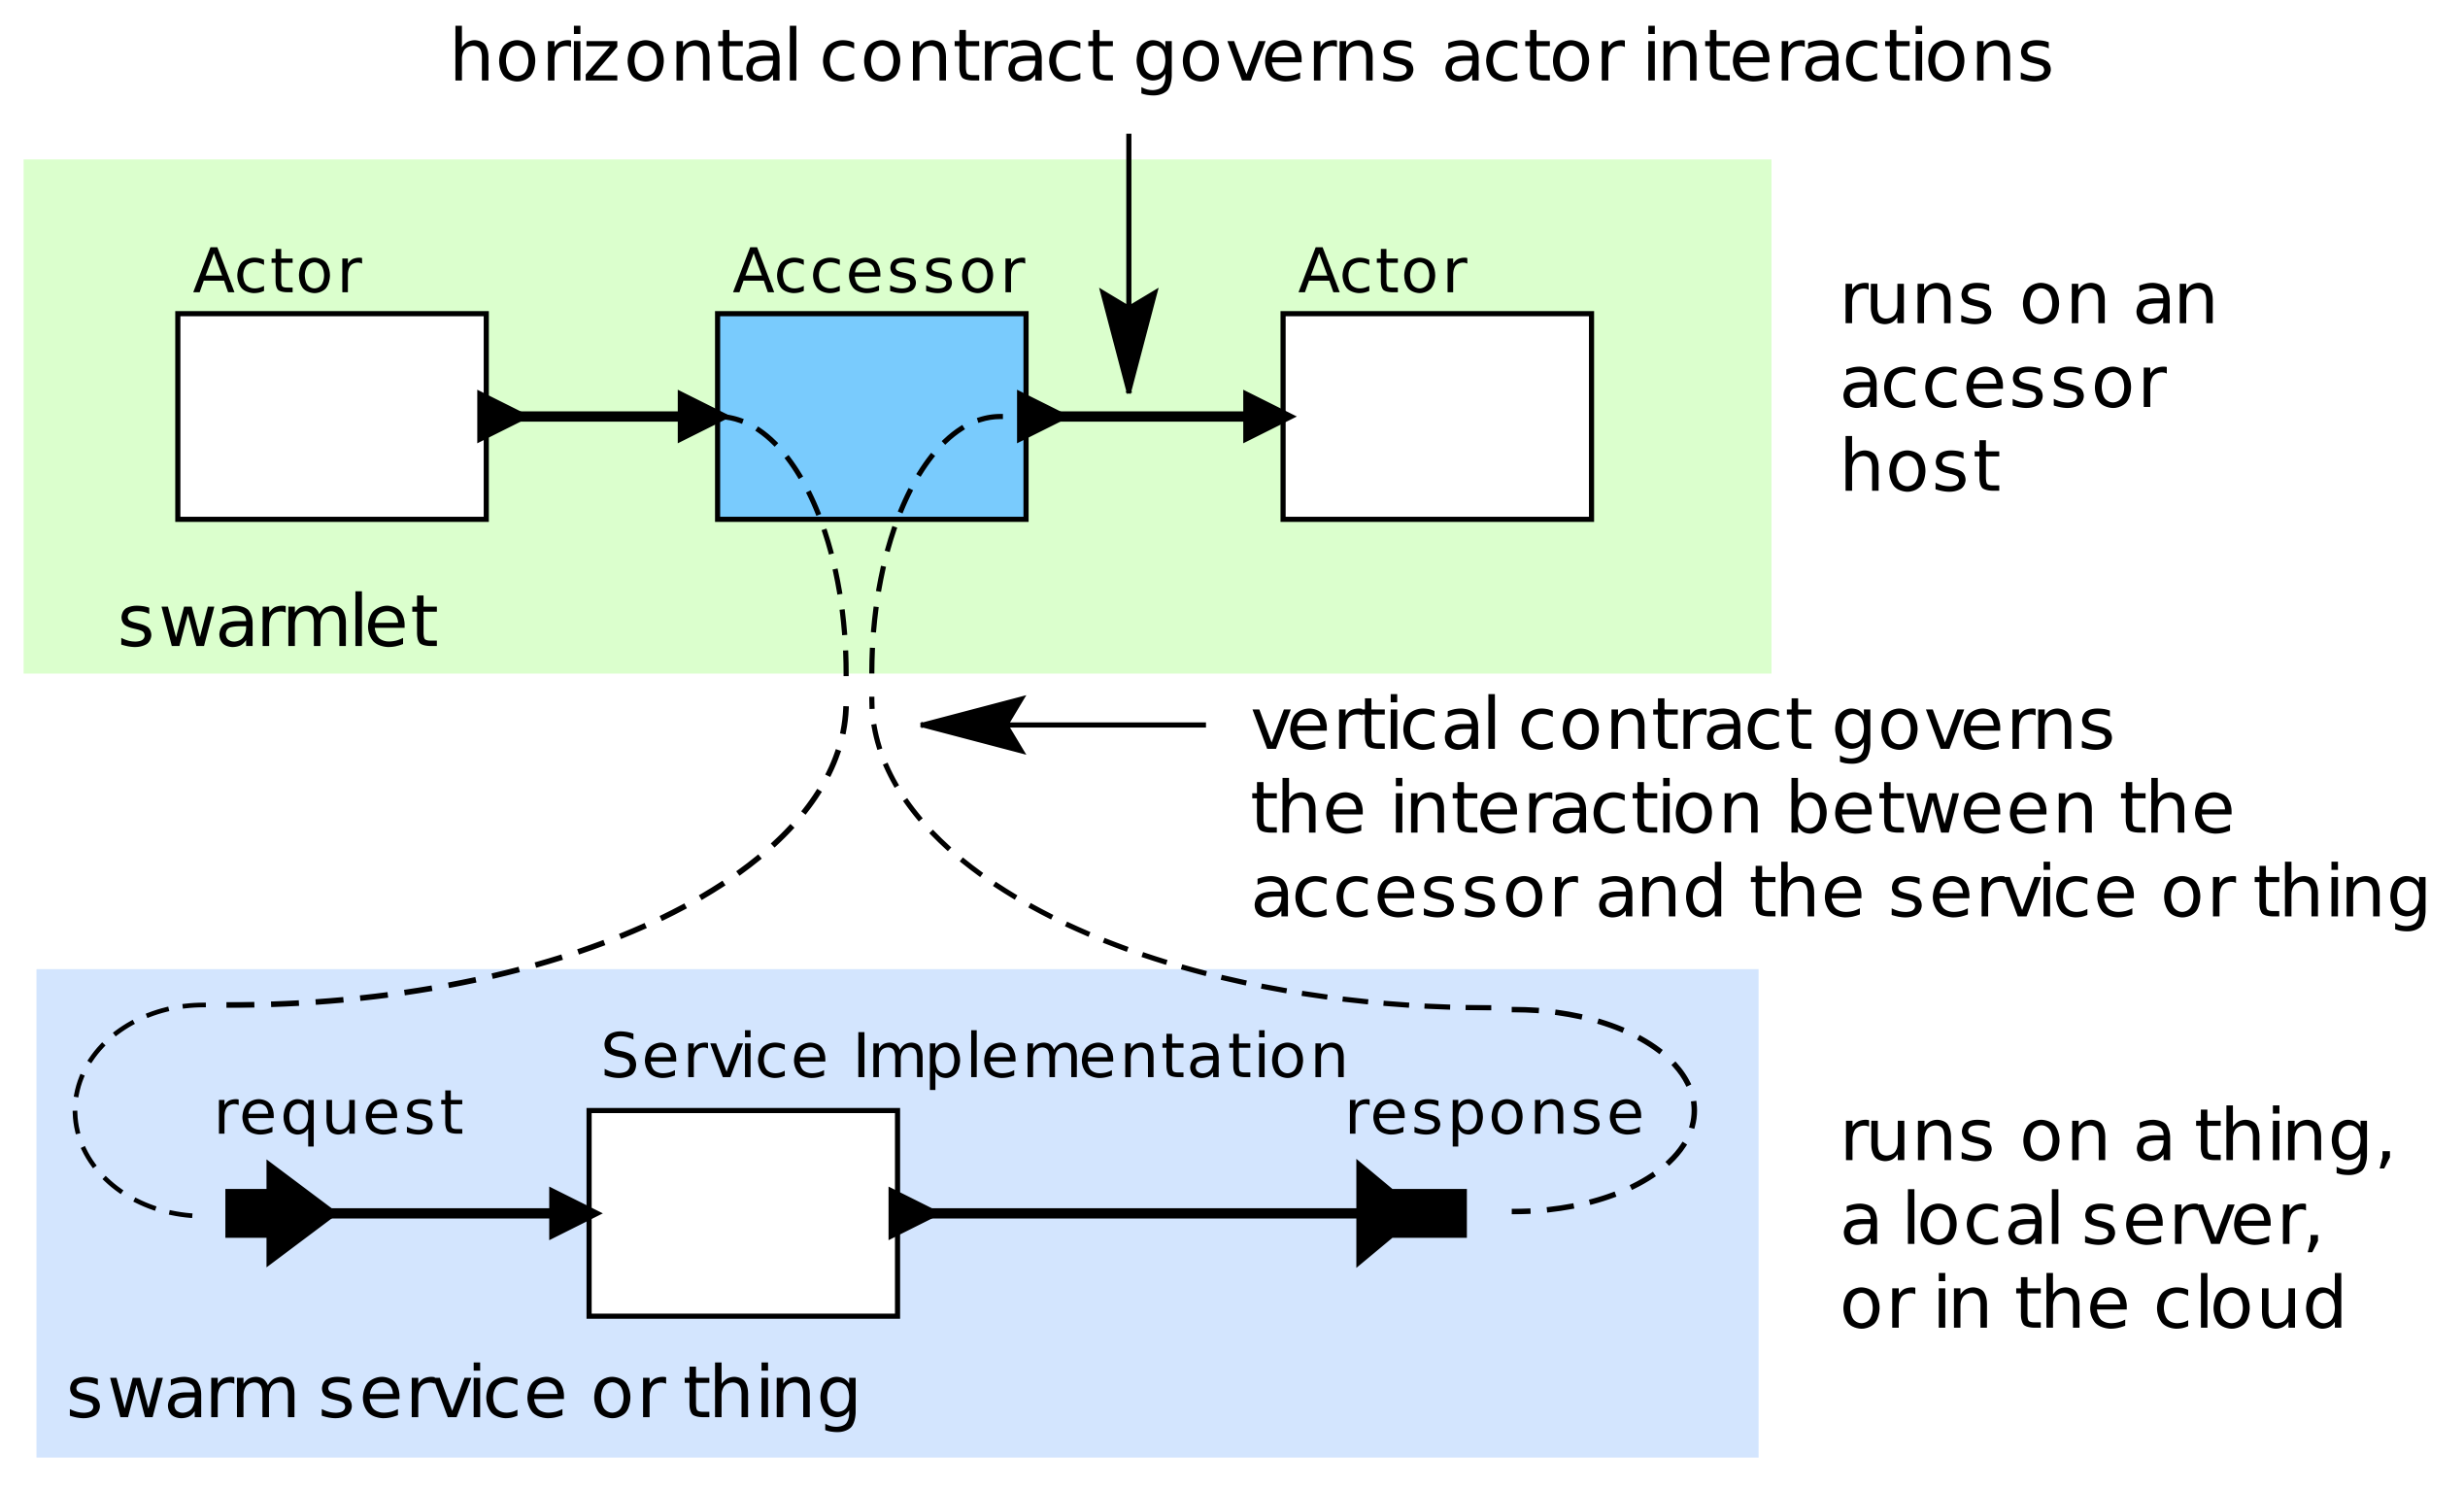
\includegraphics[height=0.4\textheight]{figures/accessors.png}
      \caption{Accessor in a network of actors.}
    \end{subfigure}
    \hfill
    \begin{subfigure}{0.49\textwidth}
      \centering
      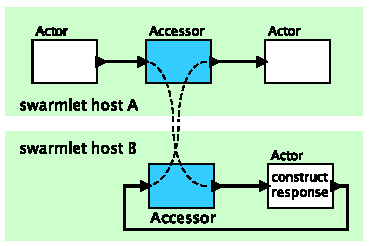
\includegraphics[height=0.4\textheight]{figures/accessors2.pdf}
      \caption{Instantiate accessors on another host.}
    \end{subfigure}
  \end{figure}

  \pause

  Work in progress with Marten and Andr\'es. Maybe checkout
  Marten's dissertation talk in the future :)
\end{frame}

%%% Local Variables:
%%% mode: latex
%%% TeX-master: "../talk"
%%% TeX-engine: xetex
%%% End:
